\documentclass[twocolumn,10pt]{asme2ej}


%% The amssymb package provides various useful mathematical symbols
\usepackage{amssymb}
%% The amsthm package provides extended theorem environments
\usepackage{graphics,graphicx,amsbsy,amssymb}
\usepackage{epstopdf}
\usepackage{float}
\usepackage{import} 
\usepackage{color} 

%% The lineno packages adds line numbers. Start line numbering with
%% \begin{linenumbers}, end it with \end{linenumbers}. Or switch it on
%% for the whole article with \linenumbers.
%% \usepackage{lineno}
% \journal{International Journal of Engineering Science}

\title{Breakup length determination of Continuous Ink Jets: application to a shear thinning industrial ink}

\author{Guillaume Ma\^itrejean
\affiliation{
    Laboratoire Rh\'eologie et Proc\'ed\'es\\
    Univ. Grenoble Alpes, LRP\\ F-38000 Grenoble France\\
    Email: guillaume.maitrejean@univ-grenoble-alpes.fr
}}

\author{Maxime Rosello
\affiliation{
    Laboratoire Rh\'eologie et Proc\'ed\'es\\
    Univ. Grenoble Alpes, LRP\\ F-38000 Grenoble France
}}
\author{Denis CD Roux
\affiliation{
    Laboratoire Rh\'eologie et Proc\'ed\'es\\
    Univ. Grenoble Alpes, LRP\\ F-38000 Grenoble France
}}
\author{Pascal Jay
\affiliation{
    Laboratoire Rh\'eologie et Proc\'ed\'es\\
    Univ. Grenoble Alpes, LRP\\ F-38000 Grenoble\\France
}}
\author{Jean Xing
\affiliation{
    Markem-Imaje Industries\\
    ZA de l'Armailler 9\\ rue Gaspard Monge\\
    BP 110 26501 Bourg-L\'es-Valence \\ France
}}
\author{Bruno Barbet
\affiliation{
    Markem-Imaje Industries\\
    ZA de l'Armailler 9\\ rue Gaspard Monge\\
    BP 110 26501 Bourg-L\'es-Valence \\ France
}}


\begin{document}
\maketitle 

\begin{abstract}
    The relaxation time of a weakly elastic polymer solution is determined by comparing numerical and experimental drop shapes. Computations use a viscoelastic Oldroyd-B model, the relaxation time of which is fitted using experimental results. This numerical approach is particularly convenient for weakly elastic solution physical parameters of which can not be measured by experimental rheometry.
\end{abstract}


%% \linenumbers

%% main text
\section{Introduction}
Capillary breakup phenomena have a wide range of applications from inkjet printing to DNA sampling. In micro jetting devices, polymer solutions often experience non
Newtonian behaviour which greatly influence breakup dynamics. Drops generation from non Newtonian fluid jets breakup is a well known topic which has already been
addressed both numerically and experimentally \cite{morrison2011inkjet,rodriguez2015experimental,mcilroy2013modelling}. Elastic and viscous effects are known to have a great influence on the breakup dynamics. More precisely, they
are known to delay the onset of the jet breakup \cite{rayleigh1892xvi, gordon1973instability}. In the present work, the relaxation time of a weakly elastic ink used in industrial continuous inkjet printing (CIJ) devices is determinated. This ink is a low viscosity dilute polymer with high polydispersity. A first estimation of the elastic relaxation time is calculated using Zimm theory \cite{zimm1956dynamics}, and is found to be out of the measurement range of both extensional rheometry (ROJER \cite{keshavarz2015studying}) or microfluidic devices \cite{galindo2013microdevices}. As a result, an original approach is introduced to determine the relaxation time, relying on the comparison of capillary breakup shapes between numerical computations and experiments.

\section{Experimental setup}
The experimental device is similar to the one used for ROJER extensional rheometry measurements \cite{rodriguez2015experimental} (see figure 1). The flow is generated by a pump and the jet is created using a micro-nozzle. Then, it is strobed at given frequency synchronized with the drive frequency ($10 kHz < f_d < 100 kHz$) in order to display a static image ($1024\times778$ pixels with $1 px \approx 1 \mu m$ ). The visualization software is ImageXpert.

\begin{figure}[H]
    \centering
    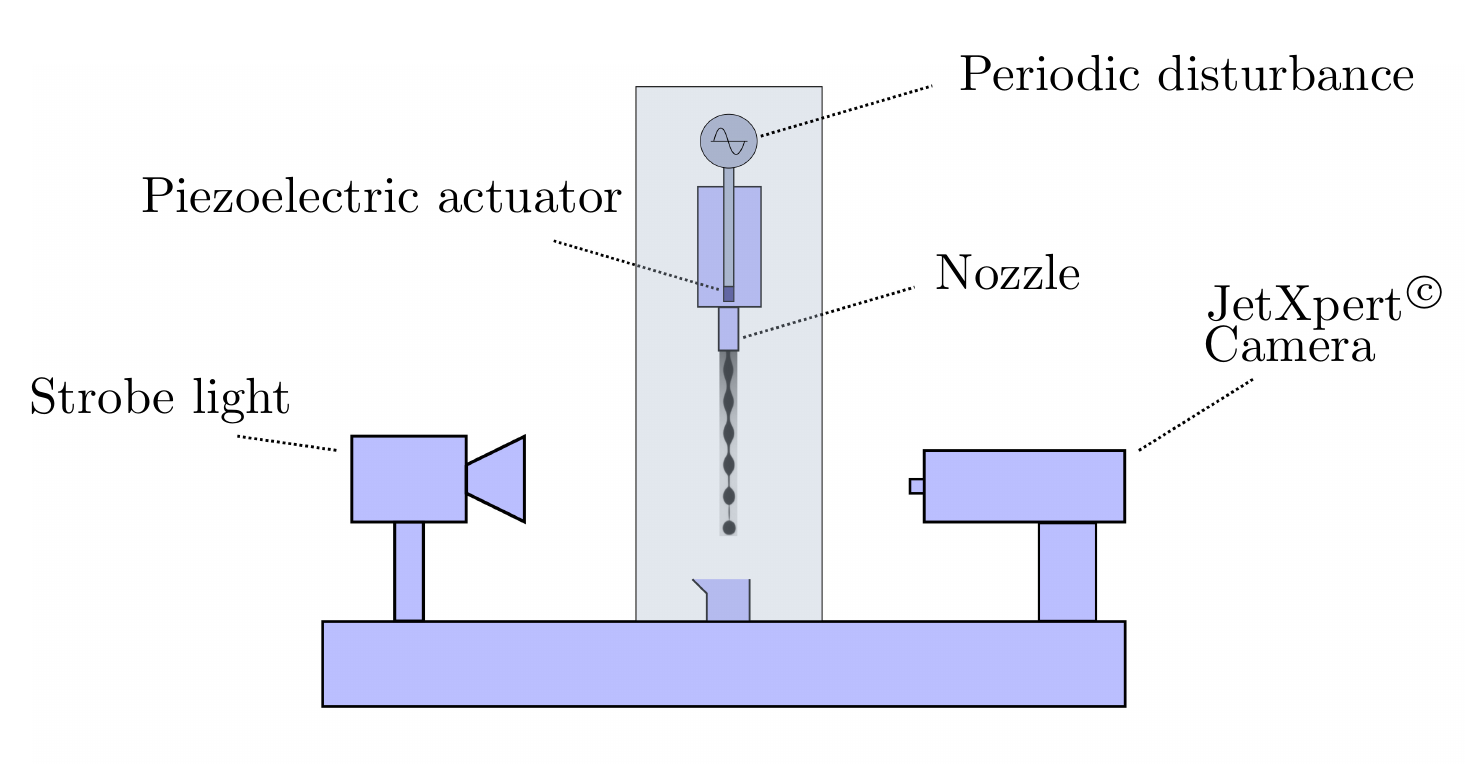
\includegraphics[width=12cm]{device.png}
    \caption{}
    \label{device}
\end{figure}

Jetting conditions are chosen to ensure a constant dimensionless wave number $x=0.6$ for all nozzles and all inks. $x$ is calculated with the wave length $\lambda$ and made dimensionless with the unperturbed jet radius $R_0$ as follow :

\begin{equation}
  x=\frac{2 \pi R_0}{\lambda}=\frac{2 \pi R_0 f}{v},
\end{equation} 

with $f$ the disturbance frequency and $v$ the undisturbed jet average velocity. Reynolds and Ohnesorge numbers, respectively $\rho U R_0 / \eta_0$ and $\eta_0/\sqrt{\rho R_0 \sigma}$ are calculated for undisturbed jets : $Re=110$ and $Oh=0.2$. These numbers are constant for every disturbance amplitudes.

Jets obtained for small disturbance amplitudes, i.e. $A_t \in [2 \, V,13 \, V]$, are  depicted Figure \ref{BUlinear}. We can see that breakup dynamics experience linear evolution and that small threads linking main drops to satellites (for instance $A_t = 13 \, V$) can be observed. These threads are typical of those observed during the breakup of weakly elastic polymer strain hardening solutions \cite{christanti2002effect}.

\begin{figure}[H] 
    \def\svgwidth{7cm} 
    \vspace{2cm}
    \centering
     \import{}{k06_5127_linear.eps_tex}
     \caption{Breakup shapes obtained in the linear regime ($A_t \in [2 \, V,13.2 \, V]$) for $x=0.6$.}
      \label{BUlinear}
  \end{figure}
 
The latter observation of viscoelasticity of the ink is consistent with its molecular composition. Indeed the ink is in the semi-dilute regime and it presents quite flexible polymer chains likely to exhibit an elastic behavior. In the next en extensive experimental study is performed to accurately determine the rheological characteristics of the ink.

\section{Rheological characterization}
Both the density $\rho = 873 kg.m^{-3}$ and the surface tension $\sigma = 22.8 mN.m^{-1}$ of the fluid have been carefully measured.

\subsection{Shear viscosity}
The shear viscosity is measured using three devices covering a wide range of shear rates, from $1s^{-1}$ to $10^6 s^{-1}$:
\begin{itemize}
    \item ARG-2 from TA-Instruments for low shear rates (from $10^0 s^{-1}$ to $10^3 s^{-1}$),
    \item a piezo-rheometer developed by \cite{buchanan2005high} for medium range shear rates (from $10^1 s^{-1}$ to $10^5 s^{-1}$),
    \item m-VROC from RheoSense for high shear rates (from $10^4 s^{-1}$ to $10^6 s^{-1}$)
\end{itemize}
As we can see on \ref{beahaviorLaw}, the viscosity can be fitted using a Cross model depicting the shear-thinning behavior:
\begin{equation}
    \eta(\dot{\gamma})=\eta_{\infty} + \frac{\eta_0 - \eta_{\infty}}{(1+\tau_{\dot{\gamma}} \dot{\gamma})^{n}},
    \label{crossEq}
  \end{equation}
where $\tau_{\dot{\gamma}}=2.10^{-7}s$ is the natural time (i.e., inverse of the shear rate at which the fluid changes from Newtonian to power-law behavior), $n=0.72$ the flow behavior index, and where finally $\eta_0=4.7 mPa.s $ and $\eta_\infty = 1 Pa.s$ are respectively the upper and lower limits of the power-law.

\begin{figure}[H]
    \centering
    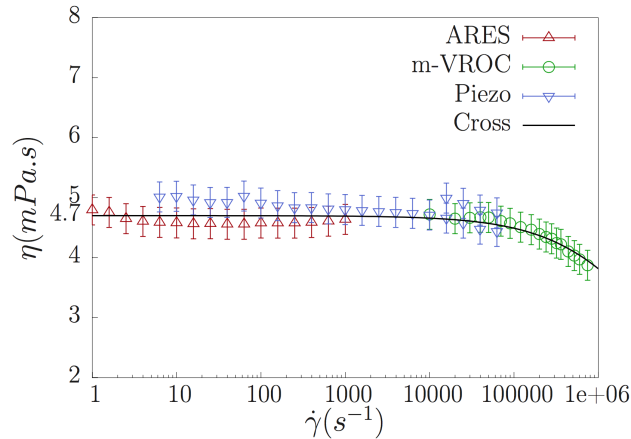
\includegraphics[width=12cm]{behaviorLaw.png}
    \caption{}
    \label{beahaviorLaw}
\end{figure}

\subsection*{Viscoelasticity}
\subsubsection*{Theoretical approach}
Elastic phenomena are characterized by stresses relaxation in the fluid. The key parameter to describe them is the polymer chain relaxation time $\lambda_p$. There is a finite number of relaxation times for each polymer in solution, each corresponding to a mode of polymer relaxation \cite{de1979scaling}. For modelling the behaviour of polymer solutions, one used to consider only the longest relaxation time corresponding to the first relaxation mode. Several microscopic analyses have been developed to calculate it according to the properties of the polymer chains.

The first theory on the subject is established by Rouse in 1953 \cite{rouse1953theory}.  The latter models the polymer chains as a succession of fixed stiffness springs and accounts only for the friction interactions between the chains. The longest relaxation time determined by this theory is rated $\lambda_R$ and is calculated via the relationship:

\begin{equation}
    \lambda_R = \frac{6 \eta_0 M}{\pi^2 \rho R T} = 0.094 \mu s,
    \label{rouse} 
\end{equation}

with $R = 8.31 \, J.mol^{-1}.K^{-1}$ the gas constant, $T$ the temperature in $K$ et $M$ the fluid molecular mass. 

This model is particularly effective in describing the behaviour of semi-dilute polymers for which interactions between chains influence the flow of the solution. However, it is less suitable for dilute polymers because it does not take into account the interactions between solvents and polymers. In the latter case, the model of Zimm \cite{zimm1956dynamics} is preferred. The latter was established in 1956 and is also based on elastic dumbbell model. It takes into account the hydrodynamic interactions between solvent and polymer chains but not the frictional interactions between chains. The only interactions between the chains are then modelled through long distance interactions mediated by the solvent. The longest relaxation time predicted by this model is calculated by:

\begin{equation}
    \lambda_Z = \frac{\eta_s [\eta] M}{RT} = 3.16 \mu s.
    \label{zimm} 
\end{equation}

Generally, and as it can be seen above, the Zimm relaxation time is more important than the Rouse relaxation time. These two models provide an effective description in different dilution regimes. However, in reality and regardless of the dilution regime, both types of interactions (chain-chain and chain-solvent) contribute to the relaxation of the chain and the present relaxation time $\lambda_p$ of the industrial ink is a compromise between the above theoretical calculations.

\subsubsection*{Relaxation time measurement}
The present jetting device can be used as a Rayleigh-Ohnesorge Jet Extensional Rheometer (ROJER) \cite{keshavarz2015studying} to directly measure the relaxation time of the present polymer solution. Hereafter a short is description of the ROJER is performed and the interested reader is invited to refer to \cite{keshavarz2015studying} and therein references for more details.
\\
The linear stability analysis of the growing Rayleigh-Plateau instability predicts a decrease of the diameter $D_P$
\begin{equation}
    \frac{D_P}{D_0}=1-\delta \, \exp(qt),
    \label{veDecay}
\end{equation}
in which $D_0$ is the initial diameter, $\delta$ is the ratio of the imposed initial perturbation to the jet diameter, and $q$ is the growth rate of the instability derived from the dispersion relation for the Rayleigh-Plateau instability for viscoelastic jet. When instability grows, the diameter of the jet no longer agrees with the linear stability and decreases in an exponential manner with the relation 
\begin{equation}
    \frac{D_P}{D_0} \sim \exp\left(\frac{-t}{3\lambda_R}\right),
\end{equation} 
where $\lambda_R$ is the relaxation time of the fluid.

The experimental results for the present polymer solution are depicted Figure \ref{Rojer}. Unfortunately the resolution of our jetting device as a ROJER is too low to observe relaxation time shorter than $\lambda_R=5.6 \, \mu s$.
\begin{figure}[H] 
    \vspace{2cm}
    \centering
     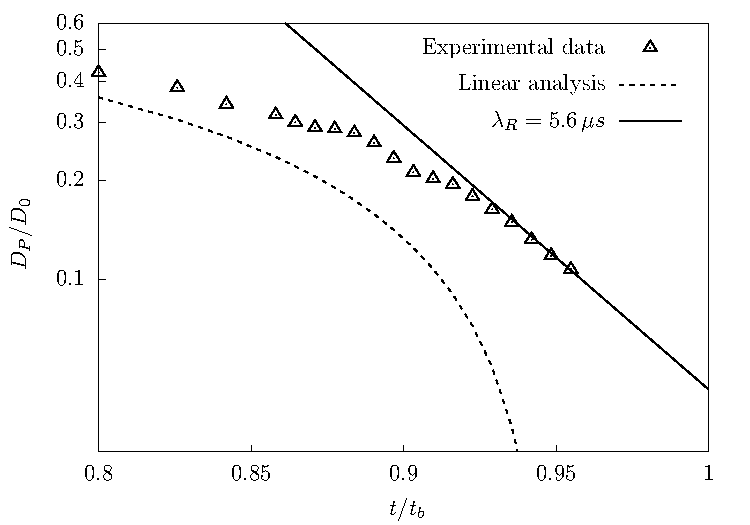
\includegraphics[width=12cm]{ROJER/rojer_bilan_zoomed.pdf}
     \caption{Decrease of dimensionless diameter $D_p/D_0$ as a function of time. Dashed line, markers and solid line depict, respectively, the result from the linear stability analysis,  experimental data and the best fit of experimental data.}
      \label{Rojer}
  \end{figure}
However, even if this measurement is not accurate enough to get the polymer chain relaxation time, it gives a first experimental upper bound.

Another route to measure the relaxation time of the polymer solution lies in the use of the oscillating piezorheometer developed by \cite{buchanan2005high}. 

\begin{figure}[H]
    \begin{center}
    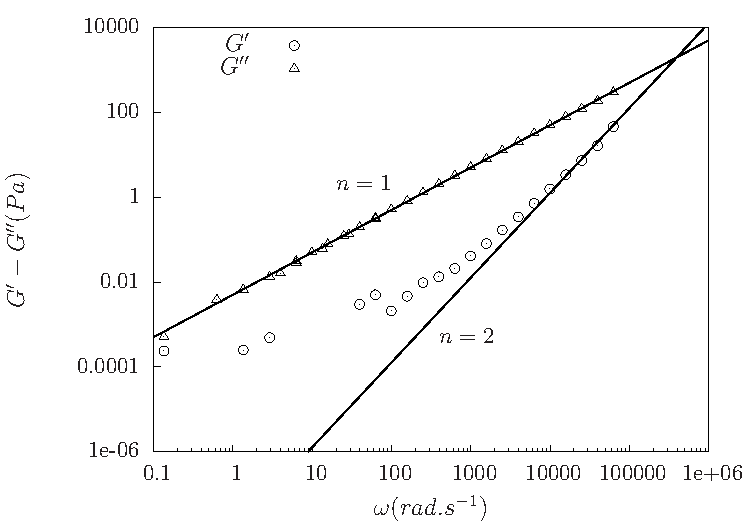
\includegraphics[width=12cm]{Moduli_bilan}
    \caption{Storage and loss modulus, $G'$ and $G''$ as a function of the piezorheometer pulsation $\omega$.}
    \label{piezo}
    \end{center}
\end{figure}

We observe for the loss module $G''$ a linear evolution over the whole oscillation range, consistent with the predictions of the Maxwell model. As for the elastic modulus, we observe an expected behavior at low frequency, i.e. the values of $ G'$ are negligible compared to those of $ G''$. However, when $\omega $ increases, we observe a progressive increase of $ G'$ which converges to a line of slope $ n = 2 $. This quadratic evolution is also characteristic of a Maxwell type relaxation, and  is consistent with a viscoelastic response. 

As expected, the experimental measurements do not allow us to observe the intersection of the moduli, it is possible to extrapolate them and get a relaxation time $ \lambda_{P} = 2.53 \, \mu s $.

It is worth noting that this value, lower than that obtained via the ROJER method, lies between Zimm and Rouse theoretical calculations.

\section{Numerical validation}

The experimental characterization of the present polymer solution gave an accurate description of of the shear viscosity but failed to accurately measure the viscoelastic relaxation time. The closest value of that relaxation time has been obtained with the piezorheometer. To assess this value numerical calculation of a 

\bibliographystyle{asmems4}
\bibliography{biblio}
\end{document}
